\section{Polymorphismus / Mehrfachvererbung / RTTI}
   	\begin{flushleft}
   	Dieses Kapitel beschreibt die dynamischen objektorientierten Sprachmerkmale von C++. Erst durch diese wird C++ zu einer echten objektorientierten Programmiersprache.
   	\end{flushleft}
	\begin{minipage}[t]{8 cm}
		\subsection{Polymorphismus \verweiscpp{14.1}}
			\subsubsection{dynamische vs. statische Bindung}
			Werden von einer Kasse A die Klassen B und C abgeleitet, so k�nnen Objekte vom Typ $Zeiger auf A$ auch auf B- oder C-Objekte verweisen. Implementieren alle drei Klassen eine Operation foo jeweils verschieden so bewirkt die Anweisung
			\lstinputlisting[language=C++,tabsize=2]{code/foo_poly.cpp}
			in normalen Programmiersprachen den Aufruf von $A::foo()$. Dabei wird bereits zur �bersetzungszeit (so fr�h wie m�glich; Early Binding) vom Compiler die Funktion $foo$ der Klasse A eingebunden. Diese Art des Bindens wird statische Bindung (static binding) genannt, da sie unver�nderbar ist. Die Variable $anAPointer$ kann in C++ auch f�r Objekte der Klasse B oder C stehen. \linebreak
			In echten objektorientierten Programmiersprache wird der obige Aufruf nicht zur �bersetzungszeit, sondern erst zur Laufzeit gebunden (dynamische Bindung, dynamic Binding). Beim Aufruf von \lstinputlisting[language=C++,tabsize=2]{code/foo_poly.cpp} wird der Typ des Objekts untersucht. In Abh�ngigkeit davon wird die Methode $A::foo$, $B::foo$ oder $C::foo$ aufgerufen. Dieses dynamische Verhalten wird als Polymorphismus bezeichnet. Damit dynamisch (zur Laufzeit) die verschiedenen Funktionen foo aufgerufen werden k�nnen, m�ssen diese Funktionen $virtual$ sein. \linebreak
	\end{minipage}\hspace*{0.5cm}
	\begin{minipage}[t]{10.5 cm}
		\subsection{Virtuelle Elementfunktionen \verweiscpp{14.2}}
			Virtuelle Elementfunktionen sind spezielle Funktionen, die nicht zur �bersetzungs- sondern zur Laufzeit gebunden werden. Es wird erst beim Auruf der Funktion entschieden, welche tats�chlich ausgef�hrt wird $A::foo$, $B::foo$ oder $C::foo$
				\begin{compactitem}
					\item Funktionen, die dynamisch gebunden werden, muss bei der Deklaration das Schl�sselwort virtual vorangestellt werden (zwingend!).
					In der abgeleiteten Klasse soll (muss aber nicht) die Funktion auch mit virtual gekennzeichnet werden. Dies sieht wie folgt aus:
						\lstinputlisting[language=C++,tabsize=2]{code/virtual.cpp}
					\item Faustregel: Eine Funktion sollte als virtual deklariert werden, wenn sie in der abgeleiteten Klasse neu definiert (�berschrieben) wird, sonst nicht!
					\item Achtung: nicht mit Funktions�berladung (gleicher Name aber unterschiedliche Signatur) verwechseln
					\item Die neue (�berschriebene) Methode muss dieselbe Signatur wie die Methode der Basisklasse haben. Sonst wird neue Methode eingef�hrt.
					\linebreak
				\end{compactitem}
	\end{minipage}
	\begin{minipage}[t]{5.5 cm}
	Im Beispiel rechts wird die Verwendung klar:
			\begin{compactitem}
				\item Der statische Datentyp bezeichnet den Datentyp bei der Deklaration. Im Beispiel: a ist ein Array von Pointer auf Article
				\item Der dynamische Datentyp bezeichnet den effektiven Datentyp zur Laufzeit Im Beispiel: a[0] ist ein Pointer auf Book, a[1] ein Pointer auf CD, etc.
			\end{compactitem}
	\end{minipage}
	\hspace*{0.5cm}
	\begin{minipage}[t]{13 cm}
		-\linebreak
		\includegraphics[width=1\textwidth]{pics/bsp_Webshop.jpg}
	\end{minipage}
\newpage
	\subsubsection{Aufruf von virtuelle Elementfunktionen \verweiscpp{14.2.2}}
	\begin{minipage}[t]{9 cm}
		Eine dynamische Methodenaufl�sung erfolgt �ber Zeiger oder Pointer:
		\lstinputlisting[language=C++,tabsize=2]{code/dynamic_call.cpp}
	\end{minipage}\hspace*{0.5cm}
	\begin{minipage}[t]{9 cm}
		Ein Aufruf mit einem Objekt und der Punktnotation wird statisch aufgel�st:
		\lstinputlisting[language=C++,tabsize=2]{code/static_call.cpp}
		Dies kommt daher, dass ein echtes Objekt sein Typ nicht ver�ndern kann (nicht polymorph) und der Compiler somit schon zur �bersetzungszeit entscheidet welche Funktion aufgerufen wird.
	\end{minipage}
	\begin{flushleft}
		Eine statische Aufl�sung wird auch erzwungen, wenn der G�ltigkeitsbereich explizit angegeben wird:
	\end{flushleft}
		\lstinputlisting[language=C++,tabsize=2]{code/static_call2.cpp}
	\begin{flushleft}
		Wichtig ist auch: innerhalb von Konstruktoren und Destruktoren \textbf{alle} Methodenaufrufe \textbf{statisch} aufgel�st werden. 
	\end{flushleft} 
	\begin{minipage}[t]{6 cm}
		\subsubsection{Polymorphe (virtuelle) Klassen}
			\begin{compactitem}
	 		\item Eine Klasse, welche mindestens eine virtuelle Funktion deklariert, heisst virtuell 	(polymorph)
			\item Virtuelle Klassen bewirken einen Mehraufwand f�r den Compiler und sind darum langsamer in der Ausf�hrung
			\item Konstruktoren sind nie virtuell
			\item Destruktoren virtueller Klassen m�ssen immer als virtuell deklariert werden,
			sonst wird nur der Destruktor der Basisklasse aufgerufen
			\textbf{ \item Nicht virtuelle Methoden d�rfen nicht �berschrieben werden} (k�nnten technisch gesehen, f�hrt aber zu un�berschaubaren Fehlern)
			\end{compactitem}
	
	\end{minipage}\hspace*{0.5cm}
	\begin{minipage}[t]{12.5 cm}
		\subsubsection{Repr�sentation polymorpher Objekte im Speicher \verweiscpp{14.2.6}}
			\begin{compactitem}
				\item In der Virtual Function Table (vtbl) vermerkt das System der Reihe nach die Adressen der f�r eine Klasse g�ltigen virtuellen Elementfunktionen
				\item Das System legt f�r jede polymorphe Klasse eine vtbl an
				\item Jedes Objekt einer polymorphen Klasse enth�lt einen Virtual Pointer vptr,
						welcher auf die vtbl der entsprechenden Klasse zeigt
			\end{compactitem}
		\hspace*{0.5cm}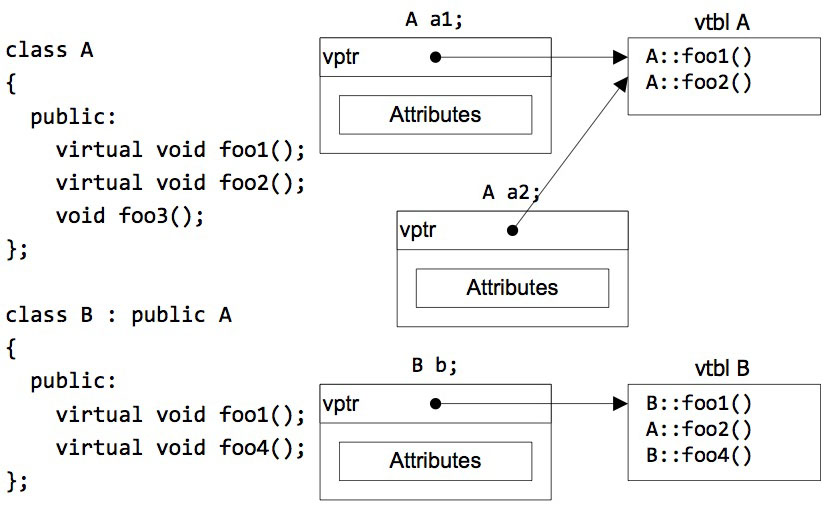
\includegraphics[width=0.85\textwidth]{pics/bsp_vtbl.jpg}
	\end{minipage}
	\subsection{Abstrakte Klassen \verweiscpp{14.3}}
		Eine abstrakte Klasse ist ein Klasse, die mehr oder weniger vollst�ndig ist und dazu dient, Gemeinsamkeiten der abgeleiteten Klassen festzuhalten (z.B. ComicCharacter). ComicCharacter legt fest, dass alle Comicfiguren die Methoden $print()$, $dance()$ und $sing()$ verstehen.
		\begin{compactitem}
			\item Ein Kreis ist z.B. ein Spezialfall einer Ellipse. Es ist aber nicht sinnvoll, ihn so zu programmieren, da er sonst Eigenschaften erbt, die nicht verwendet werden
			\item Es w�re m�glich, Kreis und Ellipse als zwei unabh�ngige Klassen zu programmieren. Dann m�ssten aber alle Eigenschaften, die diese gemeinsam haben, doppelt programmiert werden
			\item Dies versucht die objektorientierte Programmierung zu vermeiden
			\item Es ist besser, die Eigenschaften, die Kreise und Ellipsen gemein haben, in einer Basisklasse zu programmieren
			\item Die Kreis- und Ellipsenklasse erben dann parallel von der gemeinsamen Basisklasse
			\item Die Basisklasse ist aber unvollst�ndig, es handelt sich um eine abstrakte Klasse
			\item Es k�nnen \textbf{keine} Objekte von abstrakten Klassen gebildet werden
			\item In C++ k�nnen rein virtuelle Funktionen (pure virtual functions) deklariert werden, die in der Basisklasse nicht von einer Definition begleitet werden
			\lstinputlisting[language=C++,tabsize=2]{code/pure_virtual_function.cpp}
			\textbf{\item Klassen, die mindestens eine rein virtuelle Funktion deklarieren, sind abstrakte Klassen}
			\item Ist eine Klasse erst einmal als abstrakt definiert, kann diese nur durch Vererbung vervollst�ndigt und dadurch nutzbar gemacht werden
		\end{compactitem}
	
	
		